Recently, neural networks have increasingly been used to represent potentially high-dimensional probability densities or functions constrained by physical laws \cite{carleo2017solving, pfau2020ab, hermann2020deep, karniadakis2021physics, raissi2019physics, hu2023hutchinson, sun2020global}.
The physics is typically encoded in the form of partial differential equations (PDEs), and the neural network representation must therefore satisfy such equations.
This requires the application of partial differential operators to the neural network representation, which need to be computed with respect to the input rather than the trainable weights.
Unlike the setting of network training with first-order methods, these input derivatives are often high-order PDE operators, requiring second derivatives or even higher.
Efficient automatic differentiation of such operators must therefore go beyond mere backpropagation, a realization that motivated this and previous work and is illustrated in Figure \ref{fig:benchmark}.


\paragraph{Variational Monte Carlo} A prominent example is variational Monte Carlo (VMC), where neural quantum states must satisfy Schrödinger's equation \cite{carleo2017solving, pfau2020ab, hermann2020deep}.
This involves the computation of the input Laplacian to capture the kinetic energy contribution to the Hamiltonian.
In many settings, this Laplacian need not be differentiable with respect to the network weights \cite{li2023forward}.
However, recent developments in optimization techniques have also revived the use of differentiable Laplacians \cite{webber2022rayleigh, toulouse2007optimization}.

\paragraph{Physics-Informed Neural Networks} A more general framework arises in physics-informed neural networks (PINNs), which cast PDE problems as optimization tasks by minimizing the residuals of the governing equations \cite{raissi2019physics, karniadakis2021physics}.
This approach necessitates differentiable application of potentially high-order PDE operators.
For instance, the PINN formulation of Kolmogorov-type equations—including the Fokker-Planck, Black-Scholes, and Hamilton-Jacobi-Bellman equations—requires the evaluation of weighted second-order input derivatives in high-dimensional spatial domains \cite{hu2023hutchinson, sun2024dynamical}.

\paragraph{Compuational Challenges} As illustrated in Figure \ref{fig:benchmark} and Figure \ref{fig:benchmark-randomized-laplacians}, the computation of input derivatives can be a significant computational bottleneck in terms of both memory and runtime, particularly for high-dimensional or high-order operators. This limitation may restrict the scalability of recent approaches and hinder broader applicability. To address this challenge, we advocate for more efficient and automated use of advanced automatic differentiation techniques. In particular, we propose to generalize recent graph simplification strategies—such as the forward Laplacian scheme—by systematically exploiting the linearity of differential operators leveraging Taylor-mode automatic differentiation. This has the potential to both reduce resource consumption and broaden the range of feasible applications in VMC, PINNs, and related areas.

\todo{Our graphical abstract (Figure 1) is very similar to Fig.1 in \cite{li2023forward}. We can leave it as is, I just want us to be aware of it. \AW{I completely agree and would favor a different figure, also the notation is not clear at this point, I would give a }}
\newcommand{\drawgridrectangle}[4]{%
  \begin{tikzpicture}[scale=#4]
    \pgfmathsetmacro{\ymax}{#1}
    \pgfmathsetmacro{\xmax}{#2}

    % Fill the rectangle
    \fill[#3] (0,0) rectangle (\xmax,\ymax);

    % Draw the border
    \draw[white, line width=#4*3pt] (0,0) rectangle (\xmax,\ymax);


    % Draw vertical grid lines
    \pgfmathsetmacro{\xsteps}{#2}
    \foreach \x in {1,...,\xsteps} {
      \draw[white, line width=#4*3pt] (\x,0) -- (\x,\ymax);
    }

    % Draw horizontal grid lines
    \pgfmathsetmacro{\ysteps}{#1}
    \foreach \y in {1,...,\ysteps} {
      \draw[white, line width=#4*3pt] (0,\y) -- (\xmax,\y);
    }
  \end{tikzpicture}%
}

\newsavebox{\taylorStandard}
\savebox{\taylorStandard}{
  \begin{tikzpicture}
    \matrix [%
    matrix of nodes,%
    ampersand replacement=\&,% to use inside a savebox
    nodes={anchor=center, align=center},%
    column sep=4ex,%
    row sep=1ex,%
    ] (taylor)
    {
      \drawgridrectangle{1}{3}{blue!30}{0.33} \& \drawgridrectangle{1}{2}{blue!30}{0.33} \& \drawgridrectangle{1}{1}{blue!30}{0.33}
      \\[-1.5ex]
      $\vx_0$ \& $\vh_0$ \& $\vg_0$
      \\
      \drawgridrectangle{3}{3}{green!30}{0.33} \& \drawgridrectangle{3}{2}{green!30}{0.33} \& \drawgridrectangle{3}{3}{green!30}{0.33}
      \\[-1.5ex]
      $\{\vx_{1,d}\}$ \& $\{\vh_{1,d}\}$ \& $\{\vg_{1,d}\}$
      \\
      \drawgridrectangle{3}{3}{red!30}{0.33} \& \drawgridrectangle{3}{2}{red!30}{0.33} \& \drawgridrectangle{3}{1}{red!30}{0.33} \& \drawgridrectangle{1}{1}{red!60}{0.33}
      \\[-1.5ex]
      $\{\vx_{2,d}\}$ \& $\{\vh_{2,d}\}$ \& $\{\vg_{2,d}\}$ \& $\sum_d \vg_{2,d}$
      \\
    };

    % draw dependencies
    \pgfmathsetmacro{\K}{3}
    \pgfmathsetmacro{\L}{2}

    \foreach \l in {1,...,\L}{
      \pgfmathsetmacro{\lother}{int(\l+1)}
      \foreach \k in {1,...,\K} {
        \pgfmathsetmacro{\row}{int(2*\k-1)}
        \foreach \kother in {\k,...,\K} {
          \pgfmathsetmacro{\rowother}{int(2*\kother-1)}
          \draw[-Stealth, line width=1pt, white!50!black] (taylor-\row-\l.east) -- (taylor-\rowother-\lother.west);
        }
      }
    }
    \pgfmathsetmacro{\Lstart}{int(\L + 1)}
    \pgfmathsetmacro{\Lend}{int(\L + 2)}
    \pgfmathsetmacro{\rowfinal}{int(2*\K - 1)}
    \draw[-Stealth, line width=1pt, white!50!black] (taylor-\rowfinal-\Lstart.east) -- (taylor-\rowfinal-\Lend.west);
  \end{tikzpicture}
}

\newsavebox{\taylorCollapsed}
\savebox{\taylorCollapsed}{
  \begin{tikzpicture}
    \matrix [%
    matrix of nodes,%
    ampersand replacement=\&,% to use inside a savebox
    nodes={anchor=center, align=center},%
    column sep=4ex,%
    row sep=1ex,%
    ] (taylor)
    {
      \drawgridrectangle{1}{3}{blue!30}{0.33} \& \drawgridrectangle{1}{2}{blue!30}{0.33} \& \drawgridrectangle{1}{1}{blue!30}{0.33}
      \\[-1.5ex]
      $\vx_0$ \& $\vh_0$ \& $\vg_0$
      \\
      \drawgridrectangle{3}{3}{green!30}{0.33} \& \drawgridrectangle{3}{2}{green!30}{0.33} \& \drawgridrectangle{3}{3}{green!30}{0.33}
      \\[-1.5ex]
      $\{\vx_{1,d}\}$ \& $\{\vh_{1,d}\}$ \& $\{\vg_{1,d}\}$
      \\[2ex]
      \drawgridrectangle{1}{3}{red!60}{0.33} \& \drawgridrectangle{1}{2}{red!60}{0.33} \& \drawgridrectangle{1}{1}{red!60}{0.33}
      \\[-1.5ex]
      $\sum_d \vx_{2,d}$ \& $\sum_d \vh_{2,d}$ \& $\sum_d \vg_{2,d}$
      \\[1.1ex]
      \& \&
      \\
    };

    % draw dependencies
    \pgfmathsetmacro{\K}{3}
    \pgfmathsetmacro{\L}{2}

    \foreach \l in {1,...,\L}{
      \pgfmathsetmacro{\lother}{int(\l+1)}
      \foreach \k in {1,...,\K} {
        \pgfmathsetmacro{\row}{int(2*\k-1)}
        \foreach \kother in {\k,...,\K} {
          \pgfmathsetmacro{\rowother}{int(2*\kother-1)}
          \draw[-Stealth, line width=1pt, white!50!black] (taylor-\row-\l.east) -- (taylor-\rowother-\lother.west);
        }
      }
    }
  \end{tikzpicture}
}

\begin{figure*}[!t]
  \centering
  \resizebox{\linewidth}{!}{%
    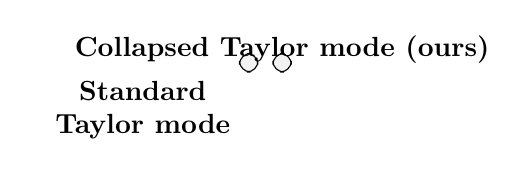
\begin{tikzpicture}
      \node (standard) [fill=black!5!white, draw=black, rounded corners]{\usebox{\taylorStandard}};
      \node [anchor=north east, align=center, inner sep=10pt] at (standard.north east) {\textbf{Standard} \\ \textbf{Taylor mode}};
      \node (collapsed) [fill=black!5!white, draw=black, rounded corners, anchor=north west, xshift=5pt] at (standard.north east) {\usebox{\taylorCollapsed}};
      \node [anchor=south, align=center, inner sep=3pt] at (collapsed.south) {\textbf{Collapsed Taylor mode (ours)}};
    \end{tikzpicture}
  }
  \caption{\textbf{Visual comparison of standard Taylor mode and our proposed collapsed Taylor mode.}}\label{fig:comparison-standard-vs-collapsed}
\end{figure*}

\begin{figure*}
  \centering
  \newsavebox{\taylorStandardNew}
  \savebox{\taylorStandardNew}{
    \begin{tikzpicture}
      \matrix [%
      matrix of nodes,%
      ampersand replacement=\&,% to use inside a savebox
      nodes={anchor=center, align=center},%
      column sep=5ex,%
      row sep=1ex,%
      ] (taylor)
      {
        \drawgridrectangle{1}{5}{gray!25!white}{0.33}
        \& \drawgridrectangle{1}{3}{gray!25!white}{0.33}
        \& \drawgridrectangle{1}{1}{gray!25!white}{0.33}
        \\[-1.5ex]
        $\vx_0$ \& $\vh_0$ \& $\vg_0$
        \\
        \drawgridrectangle{4}{5}{gray!50!white}{0.33}
        \& \drawgridrectangle{4}{3}{gray!50!white}{0.33}
        \& \drawgridrectangle{4}{1}{gray!50!white}{0.33}
        \\[-1.5ex]
        $\{\vx_{1,d}\}$ \& $\{\vh_{1,d}\}$ \& $\{\vg_{1,d}\}$
        \\[0.5ex]
        \drawgridrectangle{1}{5}{white}{0.33}
        \& \drawgridrectangle{1}{3}{white}{0.33}
        \& \drawgridrectangle{1}{1}{white}{0.33}
        \\[0.5ex]
        \\
        \drawgridrectangle{4}{5}{gray}{0.33}
        \& \drawgridrectangle{4}{3}{gray}{0.33}
        \& \drawgridrectangle{4}{1}{gray}{0.33}
        \\[-1.5ex]
        $\{\vx_{K-1,d}\}$ \& $\{\vh_{K-1,d}\}$ \& $\{\vg_{K-1,d}\}$
        \\[0.5ex]
        \drawgridrectangle{4}{5}{red!50}{0.33}
        \&
        \drawgridrectangle{4}{3}{red!50}{0.33}
        \&
        \drawgridrectangle{4}{1}{red!50}{0.33}
        \\[-1.5ex]
        $\{\vx_{K,d}\}$ \& $\{\vh_{K,d}\}$ \& $\{\vg_{K,d}\}$
        \\[-1.5ex]
        \textcolor{purple!50!red}{$\sum_d \vx_{K,d}$}
        \& \textcolor{purple!50!red}{$\sum_d \vh_{K,d}$}
        \& \textcolor{purple!50!red}{$\sum_d \vg_{K,d}$}
        \\
      };

      \node[xshift=-1pt, yshift=-14pt] at (taylor-9-1) {\drawgridrectangle{1}{5}{purple!50!red}{0.33}};
      \node[xshift=-1pt, yshift=-14pt] at (taylor-9-2) {\drawgridrectangle{1}{3}{purple!50!red}{0.33}};
      \node[xshift=-1pt, yshift=-14pt] at (taylor-9-3) {\drawgridrectangle{1}{1}{purple!50!red}{0.33}};

      \node at (taylor-5-1) {\vdots};
      \node at (taylor-5-2) {\vdots};
      \node at (taylor-5-3) {\vdots};

      % draw dependencies
      \pgfmathsetmacro{\K}{5}
      \pgfmathsetmacro{\L}{2}

      \foreach \l in {1,...,\L}{
        \pgfmathsetmacro{\lother}{int(\l+1)}
        \foreach \k in {1,...,\K} {
          \pgfmathsetmacro{\row}{int(2*\k-1)}
          \foreach \kother in {\k,...,\K} {
            \pgfmathsetmacro{\rowother}{int(2*\kother-1)}
            \draw[-Stealth, line width=1pt, gray] (taylor-\row-\l.east) -- (taylor-\rowother-\lother.west);
          }
        }
      }

      \coordinate (arrowStart) at ($(taylor-1-1.north)+(0,3.5ex)$);
      \coordinate (arrowEnd) at ($(taylor-1-3.north east)+(0,3.5ex)$);
      \draw[-Stealth, line width=2pt, black] (arrowStart) to node [midway, fill=white, align=center] {\textbf{Taylor forward} \\ \textbf{propagation}} (arrowEnd);

      \node [left=1.5ex of taylor-1-1] (zero) {0};
      \node [left=1.5ex of taylor-3-1] {1};
      \node [left=1.5ex of taylor-5-1] {$\vdots$};
      \node [left=1.5ex of taylor-7-1] {$K-1$};
      \node [left=1.5ex of taylor-9-1] {$K$};

      \node [align=center] (coefficientLabel) at ($(zero)+(0, 5.5ex)$) {\textbf{Derivative}\\\textbf{degree}};

      \draw[rounded corners] (taylor-9-1.north west) rectangle (taylor.south east);
    \end{tikzpicture}
  }

  \begin{tikzpicture}
    \node {\usebox{\taylorStandardNew}};
  \end{tikzpicture}
\end{figure*}

%%% Local Variables:
%%% mode: LaTeX
%%% TeX-master: "../main"
%%% End:



Our contributions comprise the following topics:
\begin{enumerate}
    \item We describe the `collapsed' Taylor mode where the highest Taylor coefficients during the forward propagation are propagated as a weighted sum of said derivatives.
    This approach has first been used in the `forward Laplacian framework \cite{li2023forward}, which, however, does not rely on Taylor mode.
    Our collapsed Taylor mode improves on it in two ways.
    First, it is based on standard Taylor mode that then allows simple graph rewrites based on linearity.
    Second, it generalizes to other differential operators and can also be applied to recently proposed randomization techniques for Taylor mode.

    \item This leads to a conceptually clean separation of concepts, allowing for a simple implementation that can handle all scenarios and does not require manual implementations for each differential operator.
    To demonstrate this, we build a Taylor mode library for PyTorch and equip it with the necessary graph simplifications using the \texttt{torch.fx} library, and show how collapsed Taylor mode accelerates the computation of various differential operators.

    \item Ideally, we find specially structured differential operators for which our approach is especially suited and classify them.
    One example is the trace of derivative tensors of arbitrary order, although this seems to be an operator that is not practically relevant.
\end{enumerate}

Next tasks:
\begin{enumerate}
\item @Felix: Compare Laplacian and Bi-Laplacian in JAX. 
We expect the same performance behaviors as our PyTorch results.
\item @Felix: We should say that our trick applies to computing traces of higher-order derivative tensors.
  However, we don't empirically investigate this as we do not know any use cases for such operators (yet).

\item @Tim Experiment with JAX, compare Laplacian with nested versus forward Laplacian versus using JAX.jets.experimental.
  The goal is to show that JAX's compiler is currently not capable to apply the simplifications we propose.
  @Felix push the code for preliminary experiments with JAX to the repository.
\item @Felix: Move `pedagogical' computation of the Bi-Laplacian to the appendix once we have successfully implemented the version based on Chapter 13.
\end{enumerate}

%%% Local Variables:
%%% mode: LaTeX
%%% TeX-master: "../main"
%%% End:
